\subsection{Spændingsforsyning} \label{test_spaendingsforsyning}
Det forventes, at spændingsforsyningen leverer en konstant spænding til EMG-forstærkeren på minimum $\pm 5~V$, hvilket fremgår af \autoref{EMG_krav}. For at undersøge, om spændingsforsyningen opfylder de opstillede krav i \ref{sec:krav_spaending}, testes spændingsforsyningen med et multimeter, hvor outputspændingen måles. %Ét kabel tilsluttes $V_{cc}$, og ét andet tilsuttes ground. 
Ud fra dette er den positive spænding målt til $5,574~V$ og den negative spænding til $-5,341~V$, hvilket giver en peak-to-peak-amplitude på $10,815~V$. Årsagen til at dette afviger fra de oplyste værdier i \autoref{sec:krav_spaending}, relateres til at det ikke er en ideel komponent. 

%
%Under testen, blev der ikke set udslag på multimeteret, hvorved spændingsforsyningen overholder kravet om at skulle kunne levere en konstant spænding. Dette betyder at spændingsforsyningen kan levere en spænding, som er passede for at forsyne EMG-forstærkeren.
Derudover testets der for om spændingsregulatoren signalerer et signal via en LED, hvis den ikke leverer en konstant spændingen. Under forsøget blev der anvendt nye batterier og afladede batterier. Ved at anvende nye batteriet blev det målt af spændingsregulatoren leverede en spænding på $\pm5,4~V$, hvortil LED'en lyste konstant. Ved de afladede batterier blev spænding målt til  $0,0985~mV$, hvortil LED'en ikke lyste. Dokumentation for denne test fremgår af \autoref{fig:spaendingsforsyning_LED}.


\begin{figure}[H]
\centering
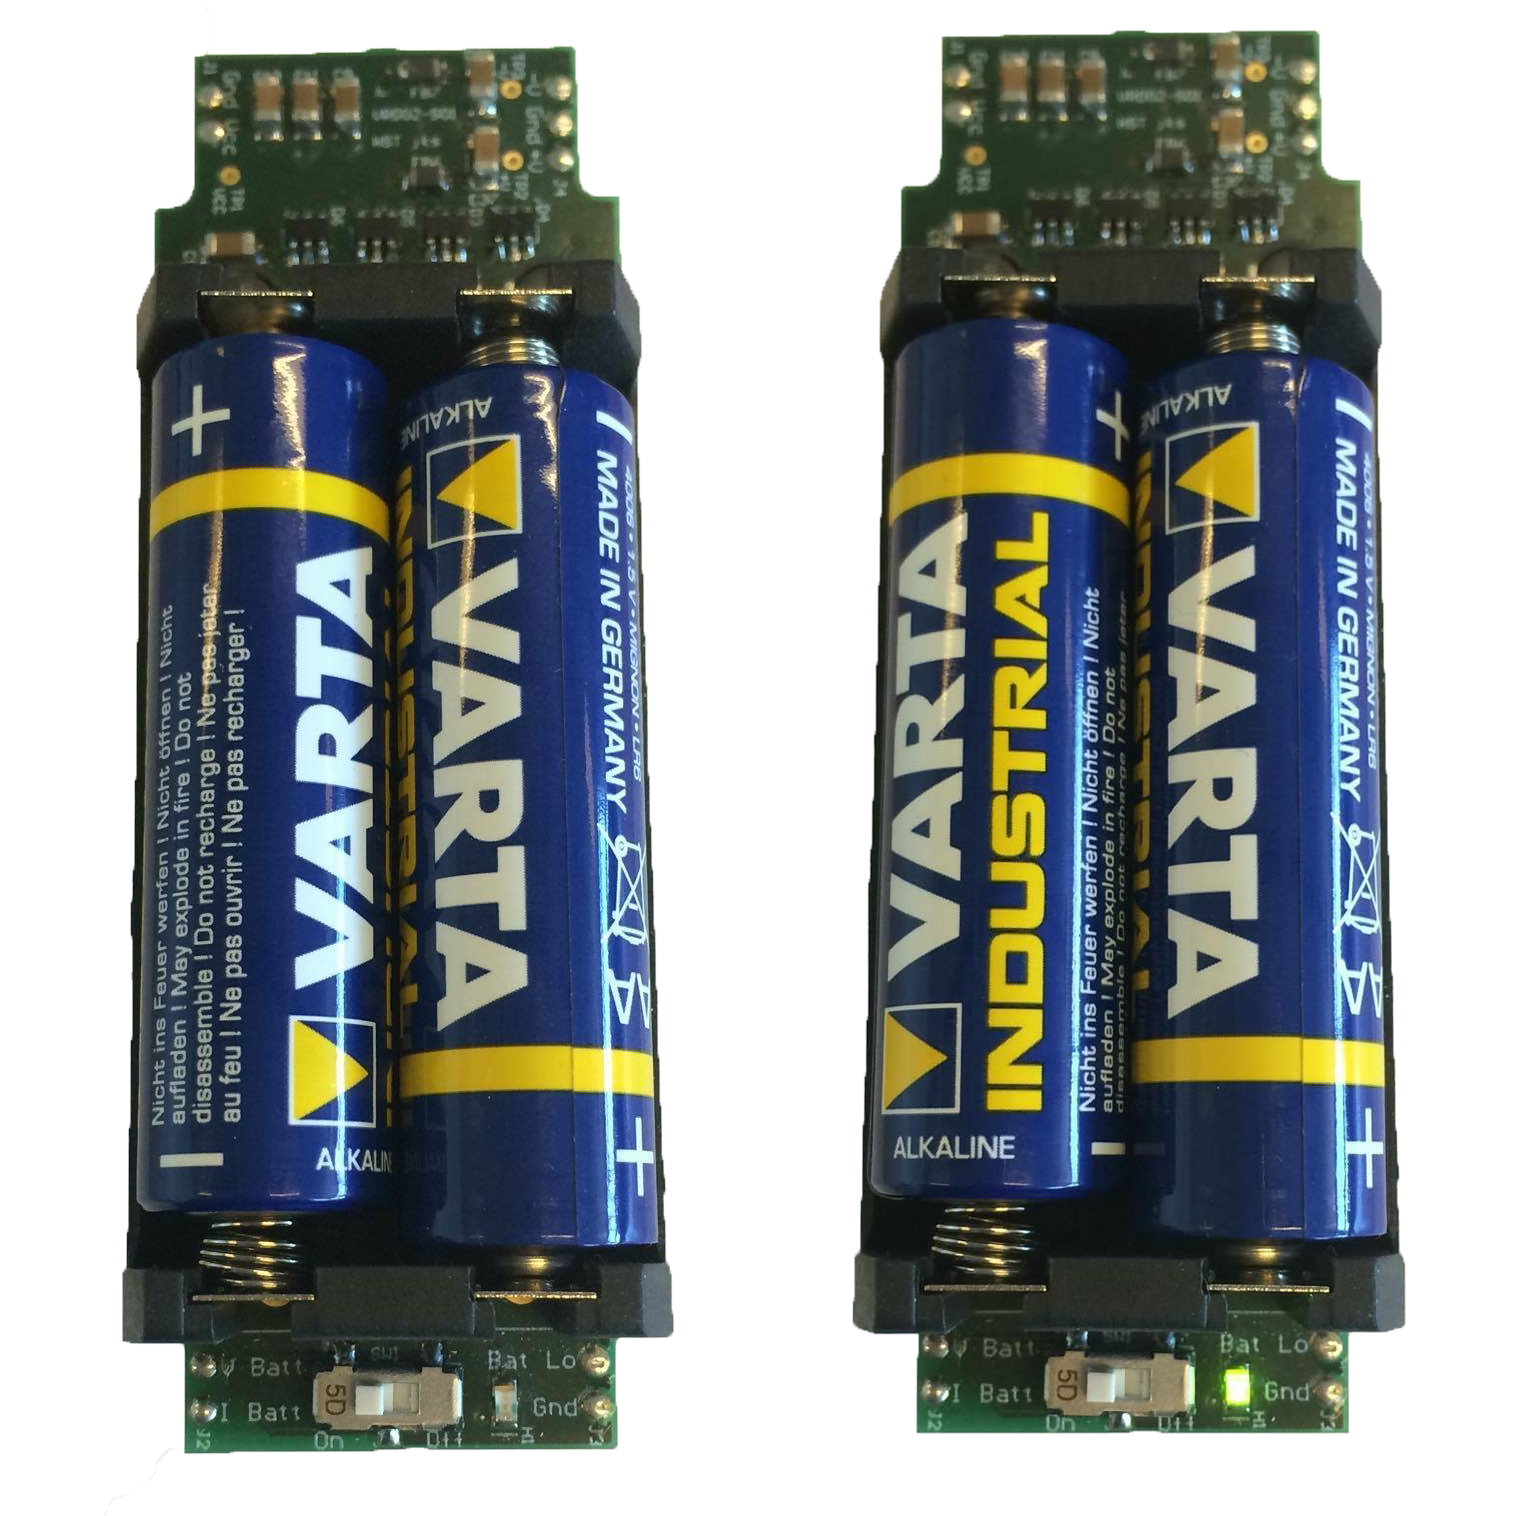
\includegraphics[width=0.6\textwidth]{figures/bat_test}
\caption{Billedet til højre viser spændingsregulatorens når den leverer en spænding på $5,4~V$, hvorved en grøn LED lyser for indikere dette. Billedet til venstre viser spændingsregulatoren når den ikke leverer en passende spænding, hvormed LED'en er slukket.}
\label{fig:spaendingsforsyning_LED}
\end{figure}

\vspace{3mm}
\textbf{Opsummering af krav:}
\begin{itemize} 
\item[\text{\sffamily \checkmark}] Skal kunne forsyne aktive komponenter i den analoge del af kredsløbet
\item[\text{\sffamily \checkmark}] Skal kunne levere en konstant spænding
\item[\text{\sffamily \checkmark}] Skal kunne give et signal, hvis der ikke leveres en konstant spænding
\end{itemize}

